\chapter{Configuration Space 位形空间}

对于机器人来说，首先要关注的是它在哪里？如何描述机器人的位置，很简单，即对机器人上的每个点做出位置描述。由于机器人的连杆是刚性且形状已知，那么仅需几个坐标就可以描述。如图，门的位置就可以用铰链的角度 $\theta$ 来描述。

\begin{figure}
    \centering
    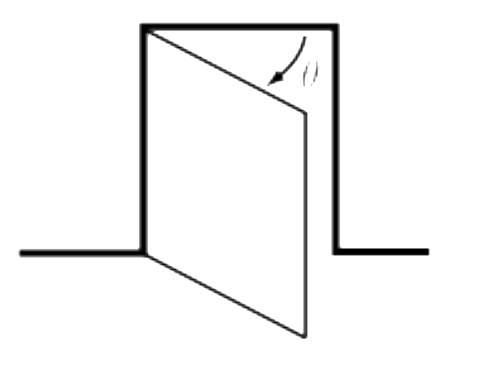
\includegraphics[width=0.3\textwidth]{Figure/门.png}
    \caption{门的位置描述}
\end{figure}

平面上某一点的位置可以用两个坐标 $(x, y)$ 来描述，硬币正面朝上放在平板上的位置可以用三个坐标来描述：两个坐标 $(x, y)$ 表示硬币上某一点的位置，角度 $\theta$ 表示硬币的朝向。这些坐标都在连续的实数域内取值。

\section{刚体的自由度}

由此，我们引出自由度的定义：\\
\textbf{机器人的自由度 ($dof$) 是表示其位形所需的最小实值坐标数。}

上述描述中，门有一个自由度，而硬币有三个自由度。需要注意，虽然硬币有正反面两种状态，但是正反面是一个离散集合，并非连续的实数空间。

\begin{tcolorbox}[colback=gray!5,colframe=black,title=C-空间定义]
The n-dimensional space containing all possible configurations of the robot is called the configuration space (C-space). The configuration of a robot is represented by a point in its C-space.
\end{tcolorbox}

包含机器人所有可能构型的高维空间称为构型空间（C-空间）。机器人的构型由其在 C-空间中的一个点来表示。

\subsection{自由度的计算推导}
以放在桌面上的硬币为例，在其上选择三个点 $A, B, C$，建立直角坐标系 $o-xy$。若点可以独立放置，硬币将有 6 个自由度。但 $A, B, C$ 三点距离为定值：
\begin{align}
    d(A,B) &= \sqrt{(x_A-x_B)^2+(y_A-y_B)^2}=d_{AB} \\
    d(C,B) &= \sqrt{(x_C-x_B)^2+(y_C-y_B)^2}=d_{BC} \\
    d(A,C) &= \sqrt{(x_A-x_C)^2+(y_A-y_C)^2}=d_{AC}
\end{align}

确定硬币位置的过程：
\begin{enumerate}
    \item 首先选择 $A$ 点坐标 $(x_A, y_A)$（2个变量）。
    \item 由于约束，$B$ 点只能在以 $A$ 为圆心的圆上，仅需夹角 $\theta$ 即可确定（1个变量）。
    \item 一旦 $A, B$ 确定，$C$ 点只有两种离散位置可选（对应正反面），不增加连续变量。
\end{enumerate}
由此，硬币在平面上有三个自由度 $(x, y, \theta)$。

\begin{figure}
    \centering
    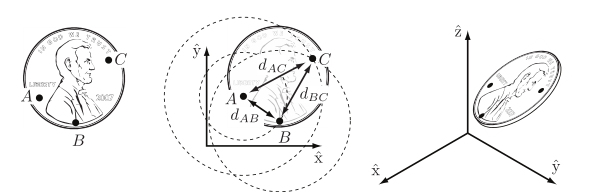
\includegraphics[width=0.8\textwidth]{Figure/自由度计算说明图.png}
    \caption{自由度计算说明图}
\end{figure}
\begin{tcolorbox}[colback=red!5!white,colframe=red!75!black]
\textbf{通用公式：}\\
自由度 = (所有点的自由度之和) - (独立约束条件数量)\\
自由度 = (变量的数目) - (独立方程的数目)
\end{tcolorbox}

\section{机器人的自由度}

考虑门：
\begin{itemize}
    \item \textbf{空间视角}：门作为空间刚体本有 6 个自由度，铰链施加了 5 个独立约束，剩 1 个自由度。
    \item \textbf{平面视角}：门作为平面刚体本有 3 个自由度，铰链施加了 2 个独立约束，剩 1 个自由度。
\end{itemize}
门的 C-空间可以用区间 $[0, 2\pi)$ 表示。

\subsection{机器人关节类型}

\begin{enumerate}
    \item \textbf{转动副 (Revolute joint, R)}: 绕轴旋转。
    \item \textbf{移动副 (Prismatic joint, P)}: 沿轴线平移。
    \item \textbf{螺旋副 (Helical joint, H)}: 绕轴同时旋转和平移。
    \item \textbf{柱副 (Cylindrical joint, C)}: 允许旋转和平移。
    \item \textbf{万向节 (Universal joint, U)}: 由一对转动副组成。
    \item \textbf{球铰 (Spherical joint, S)}: 类似肩关节。
\end{enumerate}

\begin{figure}[H]
    \centering
    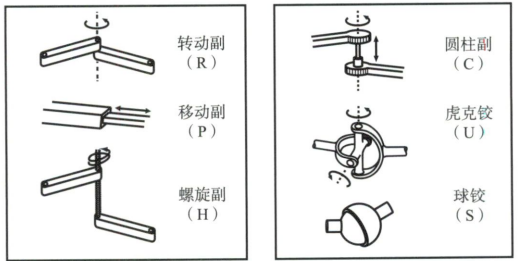
\includegraphics[width=0.8\textwidth]{Figure/典型的机器人关节.png}
    \caption{典型的机器人关节}
\end{figure}

\begin{table}
    \centering
    \caption{关节自由度与约束度对照表}
    \begin{tabular}{lccc}
        \toprule
        关节类型 & 自由度 $f$ & 平面刚体约束度 $C$ & 空间刚体约束度 $C$ \\
        \midrule
        转动副 (R) & 1 & 2 & 5 \\
        移动副 (P) & 1 & 2 & 5 \\
        螺旋副 (H) & 1 & N & 5 \\
        圆柱副 (C) & 2 & N & 4 \\
        万向节 (U) & 2 & N & 4 \\
        球铰 (S)   & 3 & N & 3 \\
        \bottomrule
    \end{tabular}
\end{table}
（还有其他很多情况）\\

\subsection{库兹巴赫公式}
\begin{tcolorbox}[colback=red!5!white,colframe=red!75!black]
\textbf{库兹巴赫公式：}对于一个具有$N$个构件的机构，令$J$为关节数，$m$为刚体的自由度数。$f_i$为关节$i$对应的自由度数，$c_i$为其对应的约束数。对于所有的$i$，始终满足$f_i+c_i=m$，则有库兹巴赫公式可写成\\
\begin{equation}
\begin{aligned}
    \text{dof} &= \underbrace{m(N-1)}_{\text{刚体自由度数}} - \underbrace{\sum_{i=1}^{J} c_i}_{\text{关节约束数}} \\
    &= m(N-1) - \sum_{i=1}^{J} (m - f_i) \\
    &= m(N-1-J) + \sum_{i=1}^{J} f_i
\end{aligned}
\end{equation}
上述公式只有在{\color{red}\text{所有}}关节都是{\color{red}\text{独立}}的情况下才能成立。否则该公式只能用于判断自由度数的{\color{red}\text{下限值}}。
\end{tcolorbox}

\section{位形空间：拓扑与表达}
\subsection{位形空间的拓扑结构}
\begin{tcolorbox}[colback=gray!5,colframe=black,title=拓扑等效]
    如果两个表面能够连续从一种形状变化到另一种形状（不能采用切割或黏结的方式），我们称之为拓扑等效。

\end{tcolorbox}


\begin{tcolorbox}[colback=red!5!white,colframe=red!75!black]
空间拓扑是空间本身的基本特性，它与我们选择的表达空间内的参考系无关。即参考系的选取不影响空间本身。
\end{tcolorbox}
\begin{tcolorbox}[colback=gray!5, colframe=black, title=C-空间的笛卡儿积（Cartesian Product）表示]
一些 C-空间可以表示成两个或者更多低维空间的笛卡儿积形式。即 C-空间的一点可以表示成低维空间点的组合：
\begin{itemize}
    \item \textbf{平面刚体}：C-空间为 $\mathbb{R}^2 \times S^1$（由位置 $(x, y) \in \mathbb{R}^2$ 和朝向 $\theta \in S^1$ 组成）。
    \item \textbf{PR 机器人}：C-空间为 $\mathbb{R}^1 \times S^1$（若考虑关节限位，则是两个封闭线段的笛卡儿积）。
    \item \textbf{2R 机器人}：C-空间为 $S^1 \times S^1 = T^2$（$T^2$ 为二维圆环面）。注意 $n$ 个 $S^1$ 的乘积等于 $T^n$，而非 $S^n$。
    \item \textbf{携带 2R 臂的移动平台}：C-空间为 $\mathbb{R}^2 \times S^1 \times T^2 = \mathbb{R}^2 \times T^3$。
    \item \textbf{三维空间刚体}：位形可描述为 $\mathbb{R}^3 \times S^2 \times S^1$ 中的一个点。
\end{itemize}
\end{tcolorbox}

\subsection{位形空间的表达}
尽管我们对于空间的描述并不会对空间本身产生影响（呵呵，渺小的我们），但为了方便计算，给出位形空间的表达是非常重要的。下面我们来看看怎么进行位形空间的表达。

\begin{tcolorbox}[colback=orange!5!white, colframe=orange!75!black, title=位形空间的表示与奇异性（Singularity）]
使用经纬度等显式参数化表示球面时，在北极或南极附近会产生\textbf{奇异性}（极小的位移引起坐标巨大变化，导致速度趋近无穷大）。为解决此问题，可采用以下两种方案：

\subsection*{1. 坐标图册（Atlas）方案}
\begin{itemize}
    \item \textbf{定义}：使用多个相互重叠且无奇异点的坐标图（Coordinate chart）覆盖整个空间。（说人话就是用$n$个坐标或参数表达$n$维空间）
    \item \textbf{优点}：总是采用最少数量的图册表示。
    \item \textbf{缺点}：需要额外的簿记工作来实现坐标图转换与规避奇异点。
\end{itemize}

\subsection*{2. 隐式表示（Implicit Representation）方案}
\begin{itemize}
    \item \textbf{定义}：将 $n$ 维空间嵌入更高维的欧氏空间中，通过约束方程减少自由度。例如单位球表示为 $x^2 + y^2 + z^2 = 1$。
    \item \textbf{优点}：无奇异性；对于闭链机构，找到其隐式表达（闭环方程）相对容易。
    \item \textbf{应用}：旋转矩阵（使用 9 个参数、满足 6 个约束方程来表示 3 个姿态自由度）可实现无奇异描述。（这个确实。别用欧拉角之类的就不会奇异？矩阵都可逆？这本书在瞎说什么。。。。让我去考证考证）
\end{itemize}
\end{tcolorbox}
\newpage
\begin{figure}
    \centering
    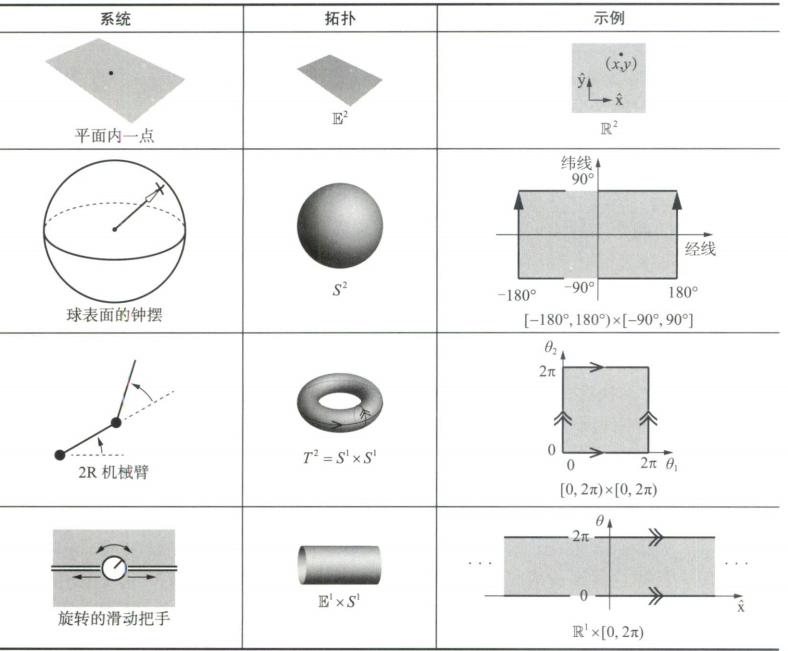
\includegraphics[width=1.0\textwidth]{Figure/几种常见拓扑结构及其坐标表示.png}
    \caption{几种常见拓扑结构及其坐标表示}
\end{figure}

\subsection{位形与速度约束}
对于含有单环或多环的机器人而言，通常使用隐式形式（Implicit Representation）比显式参数化形式更容易表达。

\subsection*{实例：平面四杆机构}
考虑如图 所示的平面四杆机构，该机构具有 1 个自由度。其四根杆总能形成一个闭环，基于几何关系可以列出以下 3 个闭环方程：

\begin{tcolorbox}[colback=blue!5!white, colframe=blue!75!black, title=四杆机构闭环方程]
\begin{align}
    L_1 \cos \theta_1 + L_2 \cos(\theta_1 + \theta_2) + L_3 \cos(\theta_1 + \theta_2 + \theta_3) + L_4 \cos(\theta_1 + \dots + \theta_4) &= 0 \\
    L_1 \sin \theta_1 + L_2 \sin(\theta_1 + \theta_2) + L_3 \sin(\theta_1 + \theta_2 + \theta_3) + L_4 \sin(\theta_1 + \dots + \theta_4) &= 0 \\
    \theta_1 + \theta_2 + \theta_3 + \theta_4 - 2\pi &= 0
\end{align}
\end{tcolorbox}

\begin{figure}
    \centering
    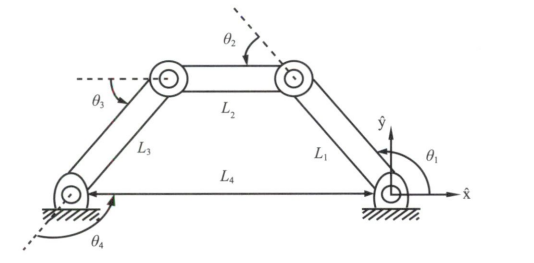
\includegraphics[width=0.6\textwidth]{Figure/four_bar_mechanism.png}
    \caption{铰链四杆机构及其坐标定义}
\end{figure}
\subsection*{推导特征与结论}
上述方程通过观察法得到，该四杆机构作为含有 4 个转动关节的闭链，具有以下几何特征：
\begin{itemize}
    \item $L_4$ 的一端与坐标原点重合；
    \item $L_4$ 总是保持水平方向。
\end{itemize}

\textbf{结论}：对于该机构，含有 4 个未知数（关节角 $\theta_1, \dots, \theta_4$）和 3 个独立方程，因此对应的所有解表示为四维关节空间中的一条一维曲线，并构成了该机器人的 C-空间。这种通过高维空间嵌入和约束方程描述的方法即为隐式表达，它有效地规避了显式参数化可能带来的奇异性问题。


\subsection{完整约束 (Holonomic Constraints)}
上述方程组可简写为 $g(\theta) = 0$。如果系统有 $n$ 个变量和 $k$ 个独立的完整约束方程，即：
\begin{equation}
\left\{
\begin{aligned}
    g_1(\theta_1, \theta_2, \dots, \theta_n) &= 0 \\
    g_2(\theta_1, \theta_2, \dots, \theta_n) &= 0 \\
    &\vdots \\
    g_k(\theta_1, \theta_2, \dots, \theta_n) &= 0
\end{aligned}
\right.
\end{equation}
则 C-空间的维数为 $n-k$。

\section{速度层面的 Pfaffian 约束推导}

对位形约束 $g(\theta) = 0$ 随时间求导，利用链式法则：
\begin{equation}
    \frac{\partial g_i}{\partial \theta_1}\dot{\theta}_1 + \frac{\partial g_i}{\partial \theta_2}\dot{\theta}_2 + \dots + \frac{\partial g_i}{\partial \theta_n}\dot{\theta}_n = 0, \quad (i=1, \dots, k)
\end{equation}

将其展开写成完整的矩阵与向量相乘的形式（Pfaffian 约束）：
\begin{tcolorbox}[colback=orange!5, colframe=orange!75!black, title=速度约束展开形式]
\begin{equation}
\begin{bmatrix}
    \frac{\partial g_1}{\partial \theta_1}(\theta) & \frac{\partial g_1}{\partial \theta_2}(\theta) & \dots & \frac{\partial g_1}{\partial \theta_n}(\theta) \\
    \frac{\partial g_2}{\partial \theta_1}(\theta) & \frac{\partial g_2}{\partial \theta_2}(\theta) & \dots & \frac{\partial g_2}{\partial \theta_n}(\theta) \\
    \vdots & \vdots & \ddots & \vdots \\
    \frac{\partial g_k}{\partial \theta_1}(\theta) & \frac{\partial g_k}{\partial \theta_2}(\theta) & \dots & \frac{\partial g_k}{\partial \theta_n}(\theta)
\end{bmatrix}
\begin{bmatrix}
    \dot{\theta}_1 \\ \dot{\theta}_2 \\ \vdots \\ \dot{\theta}_n
\end{bmatrix}
=
\begin{bmatrix}
    0 \\ 0 \\ \vdots \\ 0
\end{bmatrix}
\end{equation}
简写为：$A(\theta)\dot{\theta} = 0$。
\end{tcolorbox}

\section{非完整约束实例：滚动硬币的矩阵拆解}

对于平面滚动的硬币，位形坐标为 $q = [x, y, \phi, \theta]^T$。根据其无滑动约束，速度关系为：
\begin{equation}
\left\{
\begin{aligned}
    \dot{x} &= r \dot{\theta} \cos \phi \\
    \dot{y} &= r \dot{\theta} \sin \phi
\end{aligned}
\right.
\end{equation}



移项后，将其整理为拆开后的 Pfaffian 矩阵形式：
\begin{tcolorbox}[colback=red!5, colframe=red!75!black, title=滚动硬币约束（非完整约束矩阵）]
\begin{equation}
\begin{bmatrix}
    1 & 0 & 0 & -r\cos \phi \\
    0 & 1 & 0 & -r\sin \phi
\end{bmatrix}
\begin{bmatrix}
    \dot{x} \\ \dot{y} \\ \dot{\phi} \\ \dot{\theta}
\end{bmatrix}
=
\begin{bmatrix}
    0 \\ 0
\end{bmatrix}
\end{equation}
\end{tcolorbox}

\textbf{结论}：该约束矩阵中，通过偏微分验证可知不存在函数 $g(q)$ 使得该矩阵为其雅可比矩阵（即不可积）。因此，这属于\textbf{非完整约束}，它减少了瞬时速度自由度（由4减至2），但硬币依然可以到达四维 C-空间中的任何位置。

\section{任务空间与工作空间}

任务空间和工作空间是两个与机器人末端执行器（End-effector）位形相关的概念。需要注意的是，这两个概念均与整个机器人的位形（C-空间）无关。

\subsection{任务空间 (Task Space)}
\textbf{任务空间}是指机器人的任务能够自然表达的空间。
\begin{itemize}
    \item \textbf{定义决定因素}：任务空间完全取决于任务本身，而与机器人自身的结构无关。
    \item \textbf{示例}：
    \begin{itemize}
        \item 若任务是在纸上用钢笔画图，该任务空间为 $\mathbb{R}^2$。
        \item 若任务是操作一个刚体，则任务空间即为该刚体的 C-空间（表示附着在末端执行器上的坐标系的位姿）。
    \end{itemize}
\end{itemize}

\subsection{工作空间 (Workspace)}
\textbf{工作空间}是指机器人末端执行器所能到达位形的集合。
\begin{itemize}
    \item \textbf{定义决定因素}：工作空间主要取决于机器人的物理结构（如杆长、关节限位），而与任务无关。
    \item \textbf{与 C-空间的关系}：工作空间内的一个点可以对应多种机器人位形（多解性）。例如，一个具有 7 个关节的开链机器人，其末端执行器的 6 自由度位姿并不能完全指定机器人的唯一位形。
\end{itemize}

\begin{tcolorbox}[colback=blue!5!white, colframe=blue!75!black, title=概念对比：工作空间 vs 任务空间]
用户具有选择末端执行器部分自由度无需表示的权利。
\begin{itemize}
    \item \textbf{相同工作空间，不同 C-空间}：平面 2R 开链机械手与平面 3R 开链机械手具有相同的工作空间，尽管它们的 C-空间维数不同。
    \item \textbf{相同 C-空间，不同工作空间}：平面 2R 开链机械手的工作空间为平面圆盘，而球面 2R 开链机械手的工作空间则为球表面，尽管它们的 C-空间都是 $T^2$。
\end{itemize}
\end{tcolorbox}


\subsection{实例分析：3R 姿态调整机构}
考虑一个 3R 开链腕部机构，坐标系附着在其末端工具点处：
\begin{itemize}
    \item \textbf{工作空间}：由于末端点位置始终不变，其工作空间可定义为 3 自由度的姿态空间 $S^2 \times S^1$，这不同于其位形空间 $T^3$。
    \item \textbf{任务空间}：若任务是作为激光头（绕激光束轴线转动无关紧要），则任务空间简化为 $S^2$，表示激光所能指向的所有方向集合。
\end{itemize}

\begin{figure}
    \centering
    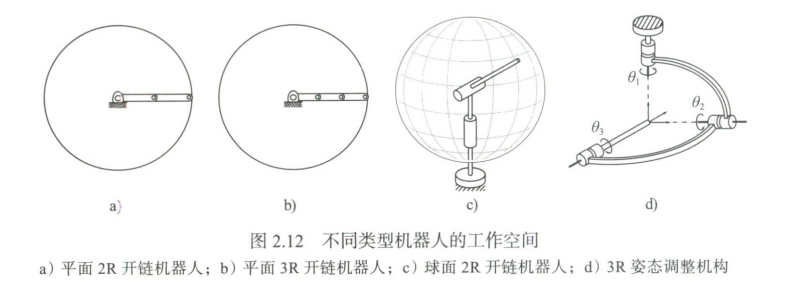
\includegraphics[width=1.0\textwidth]{Figure/不同类型机器人的工作空间.png}
    \caption{不同类型机器人的工作空间}
\end{figure}